% example with several commonly used tex constructs
\section{Design}
\subsection{Task layout}
\begin{figure}[htb]
\centering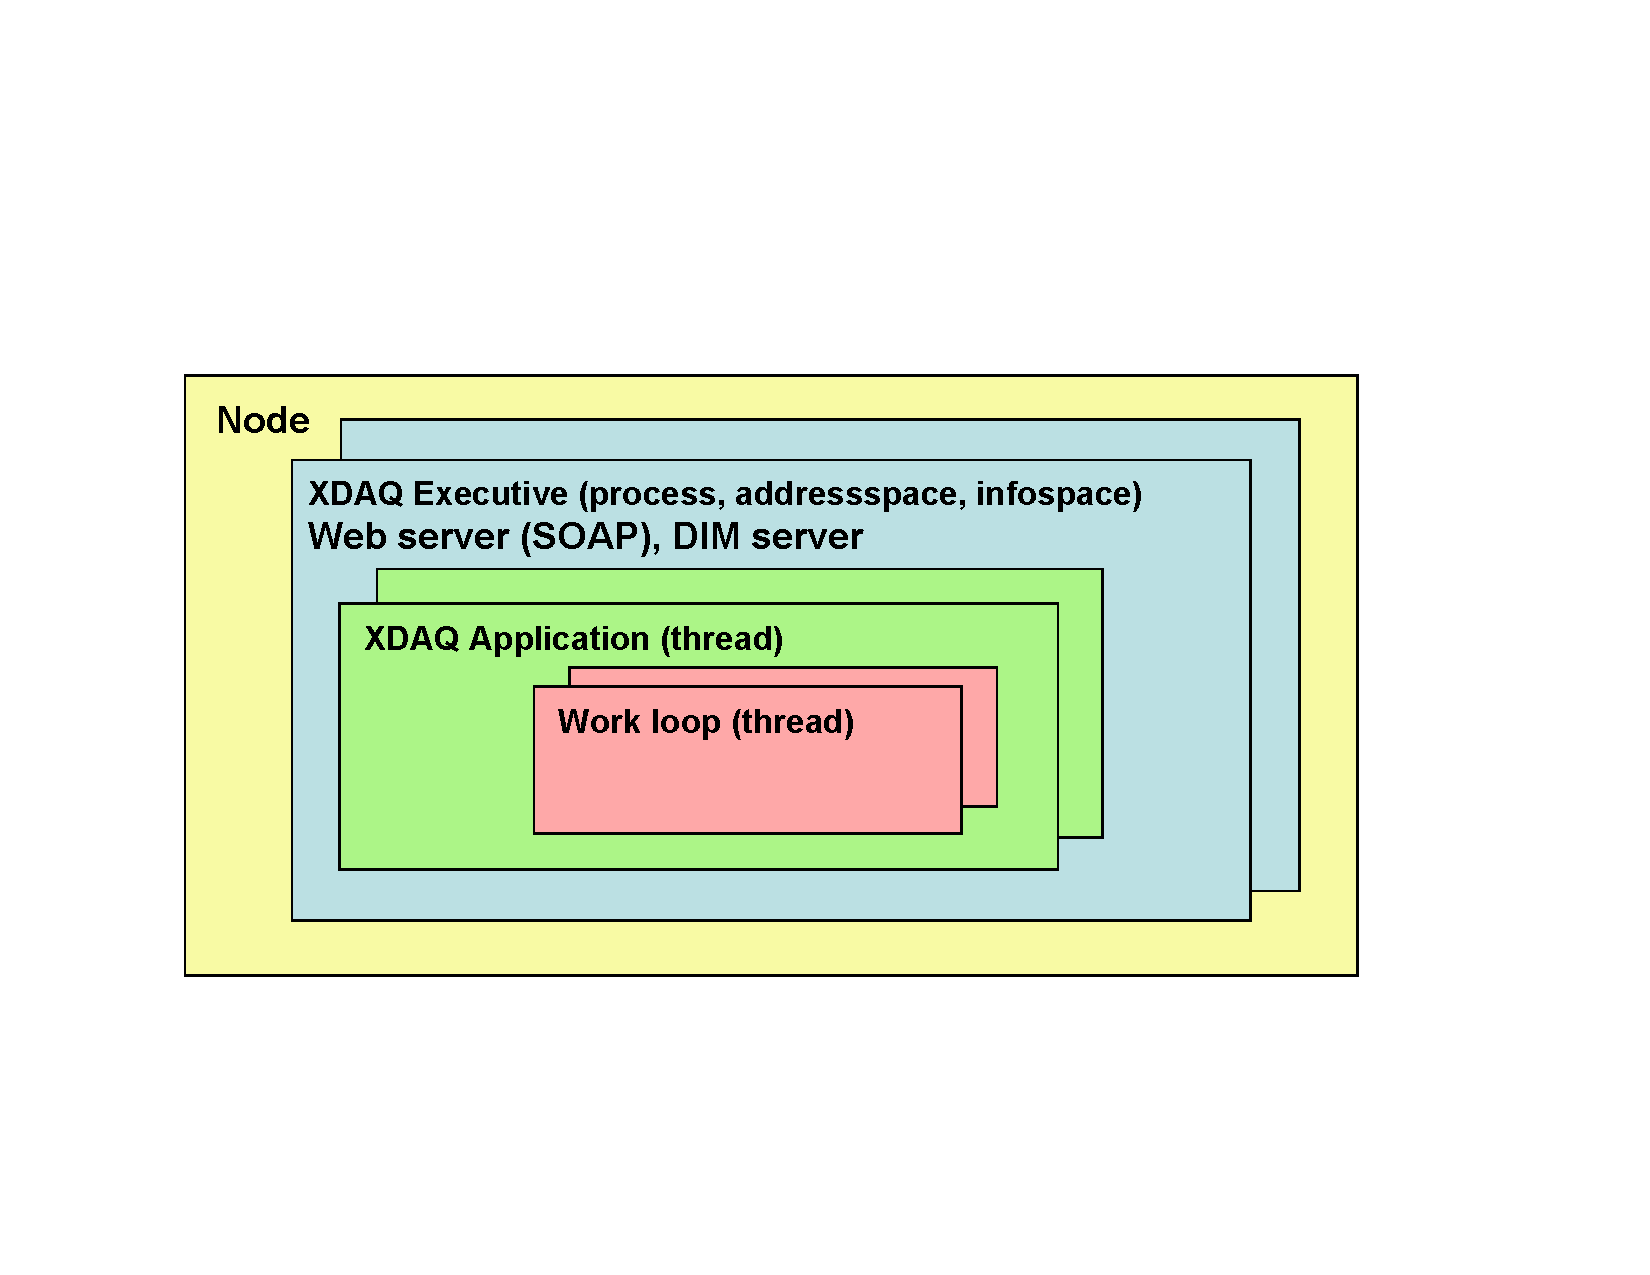
\includegraphics[width=.8\textwidth] {dabc_sw-over_3}
\caption{\xdaq~ entities} \label{fig:dabc_sw-over_3}
\end{figure}
Figure \ref{fig:dabc_sw-over_3} shows the task layout of \xdaq~.
On each node there is at least one executive which controls
the \xdaq~ applications. The applications run in threads
thus being scheduled and sharing memory. Applications also may start and
control threads (work loops).\\
The executive also is the communication stub through the Web interface or the
DIM gateway. The executive addressspace is the scope of the infospace. The
infospace provides mechanisms to access parameters across applications
and subscribe for parameter changes. The DIM gateway subscribes for
parameters in the infospace and serves them to DIM clients.\\
Figure \ref{fig:dabc_sw-over_4}, page \pageref{fig:dabc_sw-over_4} shows the data flow. There are two main
\xdaq~ executives. One runs the applications for the data input from the
front-end systems, the event building scheduler and the network senders.
The second one runs the event receiver applications for event tagging,
event building and event senders.
\clearpage
\subsection{\mbs~ data input}
\begin{figure}[htb]
\centering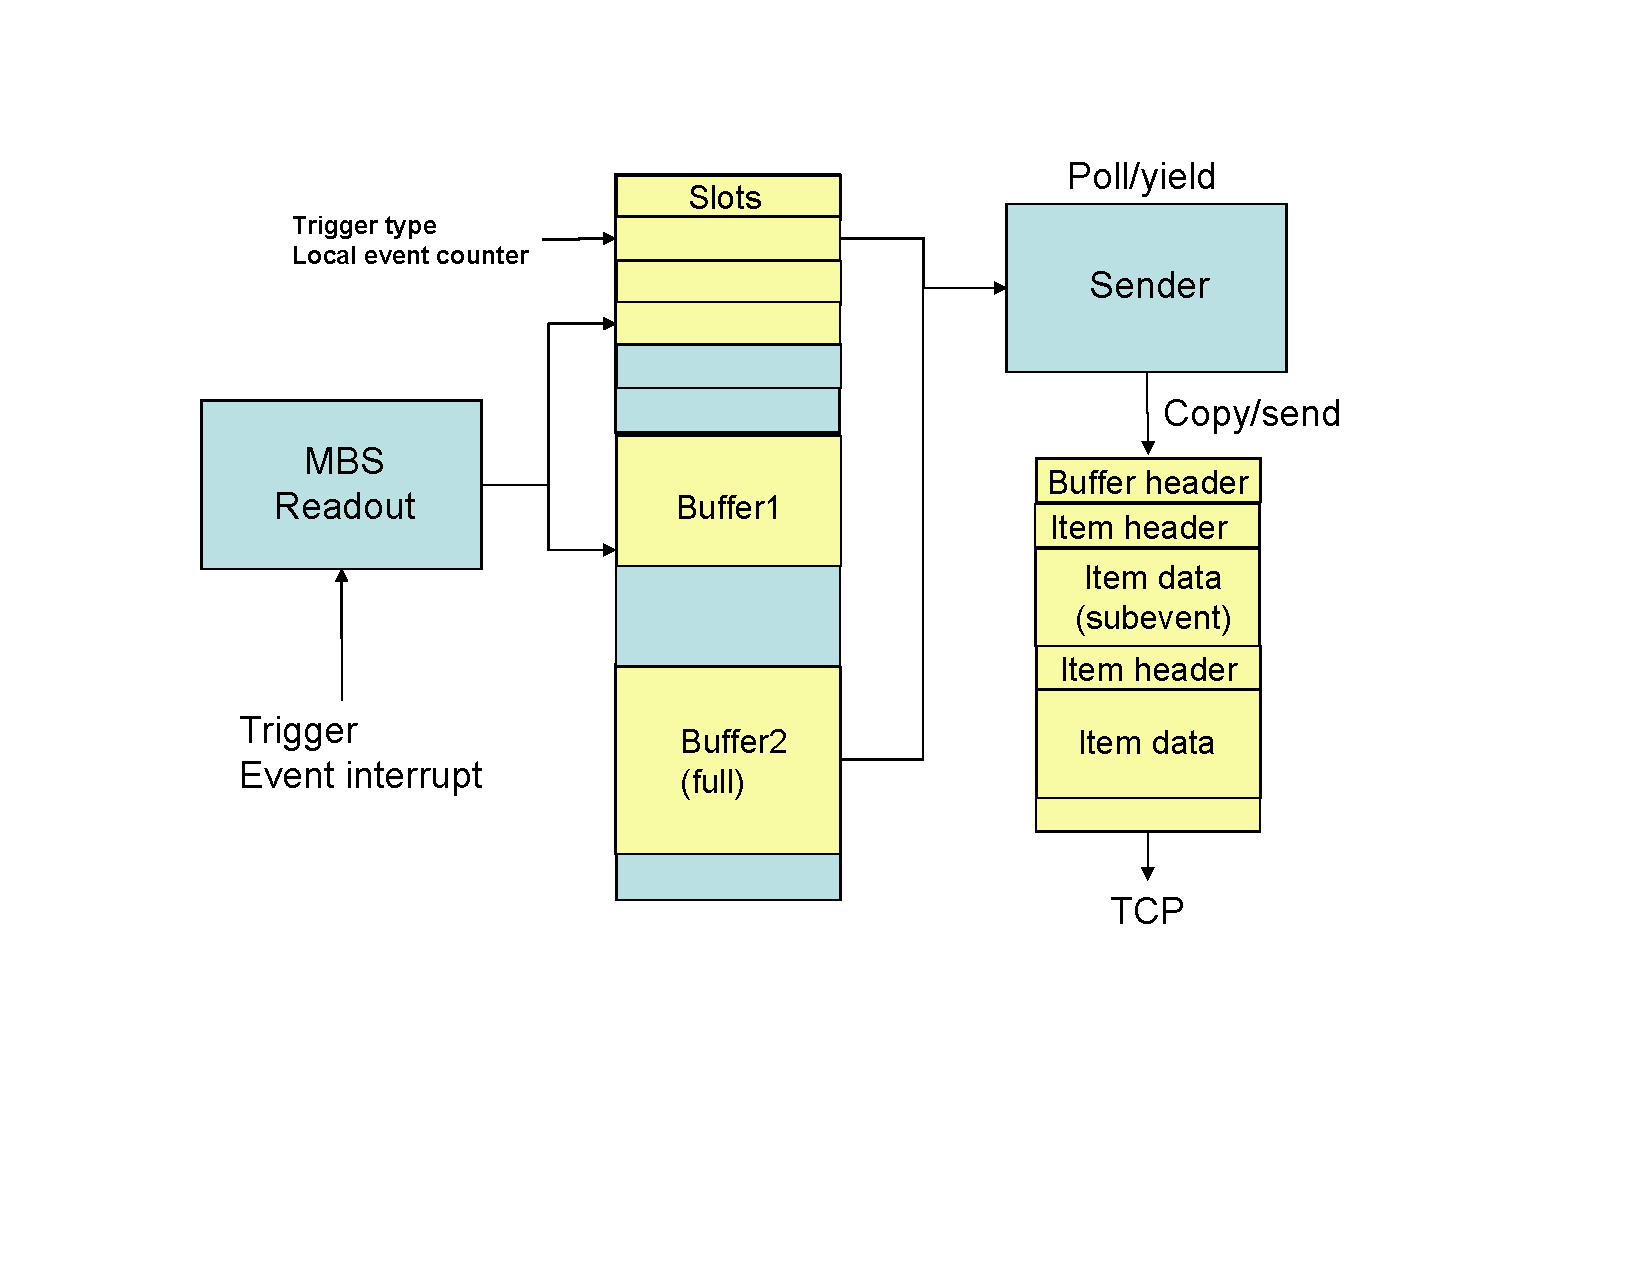
\includegraphics[width=.8\textwidth] {dabc_sw-over_5}
\caption{\mbs~ sub-event sender} \label{fig:dabc_sw-over_5}
\end{figure}
An \mbs~ data channel delivers sub-event data from one \mbs~ readout node.
On the \mbs~ side the readout task shares the sub-event pipe memory with
the sender task (see Figure \ref{fig:dabc_sw-over_5}).
The readout task receives interrupts from the trigger
module. Then it checks if there is a free slot in the pipe slot table
and enough memory in one of the two buffers. If not it yields to give
the sender the chance to empty slots. If there is a free slot and memory,
the sub-event data is read from the digitizers into the buffer. The pipe consumer,
e.g. an \mbs~ collector,
polls on ready slots, copies the sub-event data into a buffer, and frees the pipe entry.
\subsubsection{Copy mode}
Instead of the collector one can use a data sender filling a network buffer for sending
to the \dabc~ data channel (copy mode).\\
The network buffer begins with a header (endian, size, structure ID, number of items, ...).
Each item (sub-event inclusive header) has an item header keeping the
trigger type and sub-event counter (from trigger module, cyclic).\\
The logic of such a mode is very similar to the \mbs~ collector/transport (transport mode).
Therefore a \dabc~ input channel could alternatively connect to an \mbs~ transport and read LMD buffers.
The disadvantage of this logic is the performance loss due to the data copy.
In the first case, the data is more convenient for the receiver, because
it's format can be optimized for it.
In LMD buffer streams events may span over buffers. \\
\subsubsection{Zero copy mode}
\begin{figure}[htb]
\centering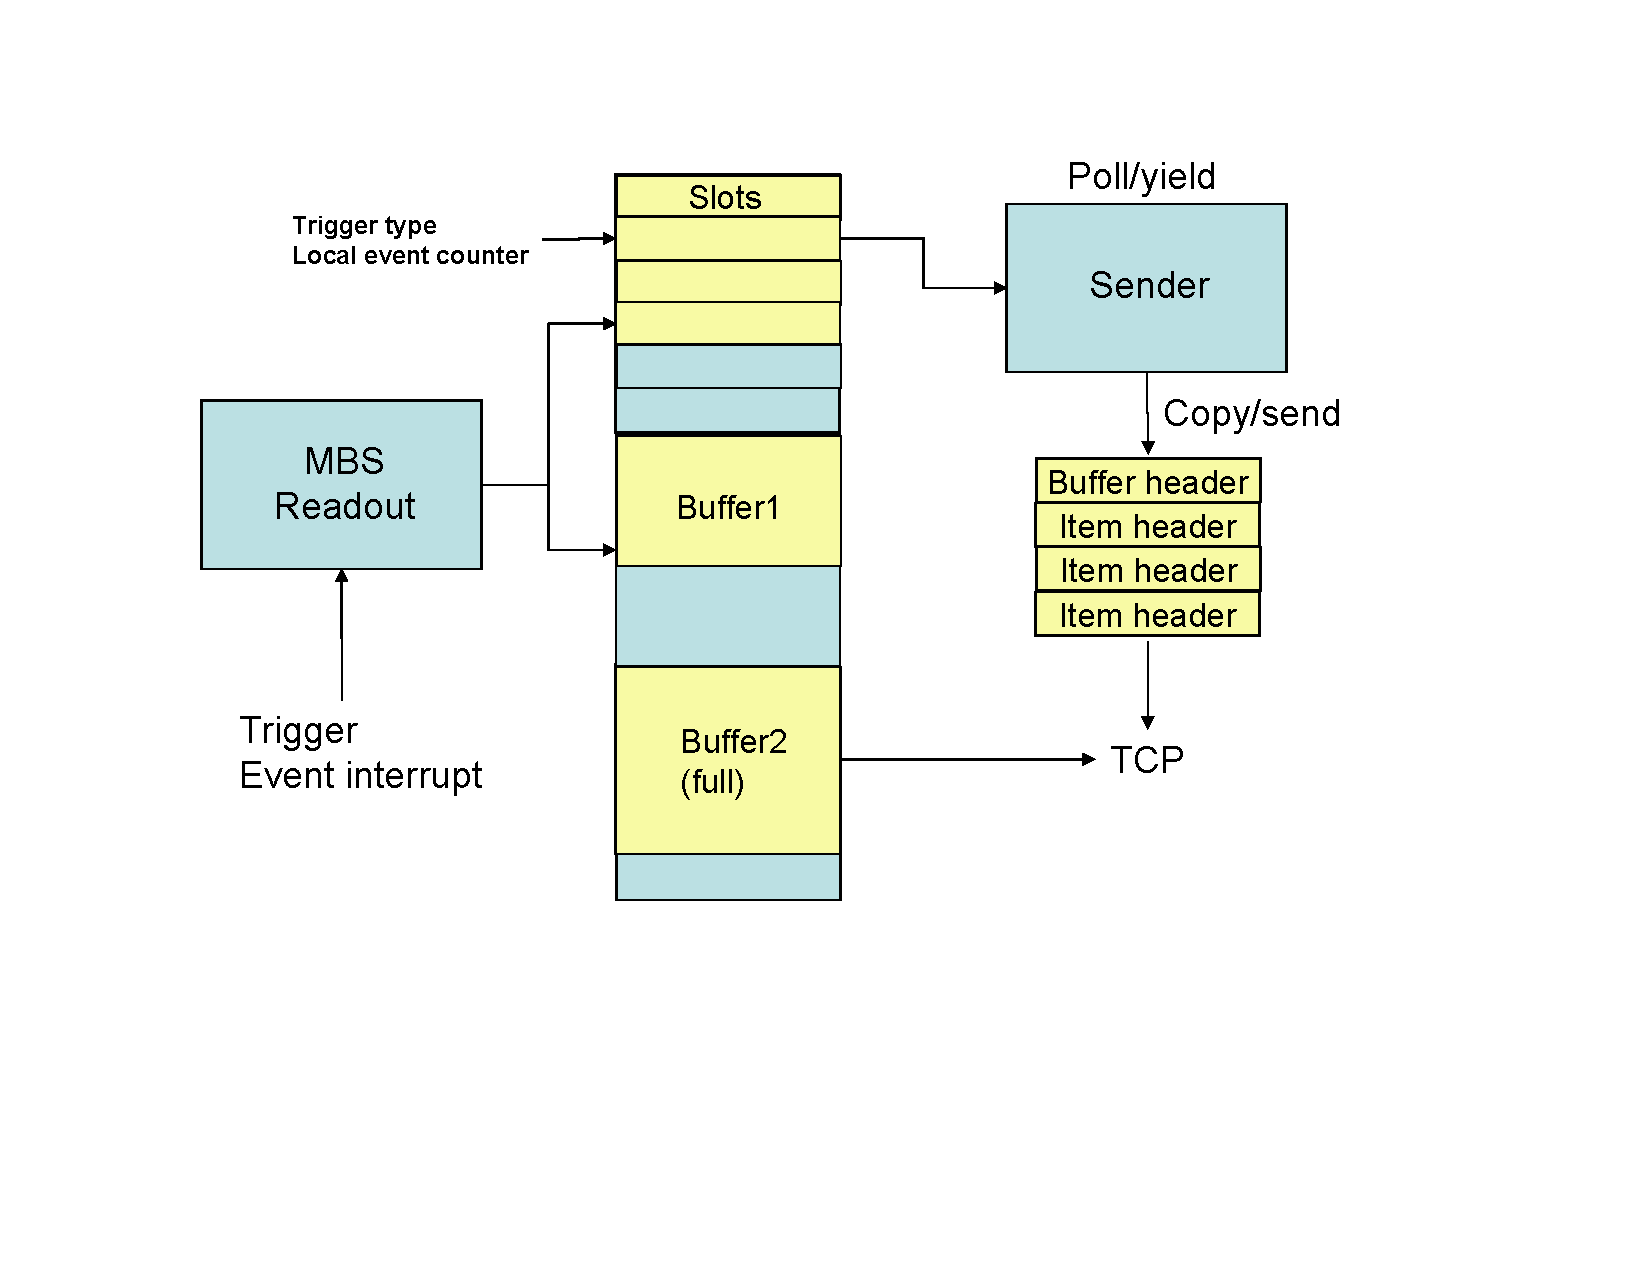
\includegraphics[width=.8\textwidth] {dabc_sw-over_6}
\caption{\mbs~ sub-event sender zero copy mode} \label{fig:dabc_sw-over_6}
\end{figure}
Another logic would not copy the data but send it directly from the pipe memory
(zero copy mode, Figure \ref{fig:dabc_sw-over_6}).
In this case a sub-event directory structure must be sent before. Each entry
keeps the trigger type and sub-event counter. In the \dabc~ input channel
the sub-event data must be combined with the directory data, i.e. copied.
A similar logic is used by the \mbs~ sub-event sender. This sender is already
optimized with the readout and could be used as base for a \dabc~sender.\\
Unfortunately the best performance logic depends on the event rate/fluctuation and
the sub-event size/fluctuation. With small sub-events at high rate logic one (copy and one TCP write per many events)
would be best, with large sub-events at low rate the last logic (one TCP write per event).
At the receiver side the difference is mainly in the data structure. A data copy
as required at least with the transport and zero copy mode will be faster than
on the front-end CPU. However, several \mbs~ input channels may run on one \dabc~node.
\subsubsection{Communication protocol}
\begin{compactenum}
\item The \dabc~ input channel connects to the \mbs~ server, either the transport or the
sender (must be started on \mbs-side) selected by port number.
\item An acknowledge message of 4 longwords is returned (endian=1, size, buffers, streams).
For transport that means that \dabc~ needs a buffer of size x buffers bytes to store all
events of a stream completely (no fragments).
\item Start reading buffers. When the reading is slower than the \mbs~ can send,
the \mbs~ blocks!\\
\mbs~ transport sends always all buffers of a stream, except empty buffers
and buffers behind the one containing the stop acquisition event.
Because \dabc~ might need to know when a stream is finished, a change in transport is
necessary to mark the last buffer of stream. For this the not used
l\_free[2] field in the buffer header might be used.
Currently it is always 0. A 1 could indicate last buffer. Events must be copied
to be contiguous in memory (because of spanning events)\\
\mbs-sender returns size=maximum, buffers=1,2 (copy, zero copy mode), streams=0.
The data buffers it sends have variable length. Therefore \dabc~ reads always
a minimum buffer (e.g. 1K) to get the actual size, and then the rest.
Depending on the mode the buffer read must be processed differently.
In copy mode the buffer probably is formatted in a way to be processed directly.
In zero copy mode the events must be merged with additional data, i.e. copied.
\item Close connection.
\end{compactenum}
The resulting format of all modes should be identical, i.e. like the copy mode:
\begin{table}[h]
\begin{tabular}{|p{2.0cm}|p{2.0cm}|p{2.0cm}|p{8.0cm}|}      \hline
Londword & \multicolumn{3}{l|}{endian=1} \\ \hline
Londword & \multicolumn{3}{l|}{structure ID} \\ \hline
Londword & \multicolumn{3}{l|}{size} \\ \hline
Londword & \multicolumn{3}{l|}{number of items} \\ \hline
Item & Longword & \multicolumn{2}{l|}{Trigger type} \\ \hline
 & Longword & \multicolumn{2}{l|}{Event counter} \\ \hline
 & Subevent & Longword & Size \\ \hline
 &  & Word & Type \\ \hline
 &  & Word & Subtype \\ \hline
 &  & Word & Processor id (from setup)\\ \hline
 &  & Byte & sub-crate \\ \hline
 &  & Byte & Processor type code \\ \hline
 &  & 3 Longword & Time stamp (optional) \\ \hline
 &  & & Data \\ \hline
\end{tabular}
\caption{Buffer structure.}
\label{dabc-mbs-buffer-table}
\end{table}


\subsubsection{\mbs~ control}
The remote \mbs~ system can be controlled completely by \dabc.
The \mbs~ is started by remote shell commands and controlled by
sending commands to the \mbs~ prompter. The controlling process
can request the \mbs~ status information.
